\section{2020 Analysis \& Differential Equations}

\subsection{Individual \& Team}

\begin{exercise}
Let $\chi$ be a real valued smooth function with compact support on $\mathbb{R}$. We assume that
\[
\int_{\mathbb{R}^1}\chi(x)\,dx = 1.
\]

For all $\varepsilon>0$, we define
\[
\chi_{\varepsilon}(x) = \frac{1}{\varepsilon}\chi\left(\frac{x}{\varepsilon}\right).
\]

Prove that for any given $f\in L^1(\mathbb{R})$, for almost every $x\in\mathbb{R}$, we have
\[
\lim_{\varepsilon\to 0}(\chi_{\varepsilon}*f)(x) = f(x).
\]

\end{exercise}

\begin{solution}
\textbf{Prerequisites:} 
\begin{itemize}
    \item \textbf{Lebesgue Differentiation Theorem:} For $f \in L^1(\mathbb{R})$, $\lim_{r \to 0} \frac{1}{2r} \int_{-r}^r |f(x-y) - f(x)| \, dy = 0$ for almost every $x$.
    \item \textbf{Approximation of the Identity:} A family of functions that "concentrates" its mass at the origin as a parameter $\varepsilon \to 0$.
    \item \textbf{Convolution Properties:} The integral $\int f(x-y)g(y)dy$ which "smears" one function with another.
\end{itemize}

\bigskip

\textbf{Steps:}
\begin{enumerate}
    \item \textbf{Express the Difference:} Using the fact that $\int_{\mathbb{R}} \chi(z) \, dz = 1$, we can write:
    \[ |(\chi_\varepsilon * f)(x) - f(x)| = \left| \int_{\mathbb{R}} \chi_\varepsilon(y) f(x-y) \, dy - f(x) \int_{\mathbb{R}} \chi_\varepsilon(y) \, dy \right| = \left| \int_{\mathbb{R}} \chi_\varepsilon(y) (f(x-y) - f(x)) \, dy \right|. \] \\[1em]
    
    \item \textbf{Change Variables:} Let $y = \varepsilon z$, so $dy = \varepsilon dz$. The integral becomes:
    \[ \left| \int_{\mathbb{R}} \frac{1}{\varepsilon} \chi(z) (f(x-\varepsilon z) - f(x)) \varepsilon \, dz \right| \leq \int_{\mathbb{R}} |\chi(z)| |f(x-\varepsilon z) - f(x)| \, dz. \] \\[1em]

    \item \textbf{Use Compact Support:} Since $\chi$ has compact support, let $\text{supp}(\chi) \subseteq [-M, M]$ and $\|\chi\|_\infty = A$. Then:
    \[ |(\chi_\varepsilon * f)(x) - f(x)| \leq A \int_{-M}^M |f(x-\varepsilon z) - f(x)| \, dz. \] \\[1em]

    \item \textbf{Apply Lebesgue Differentiation Theorem:} Let $h = \varepsilon z$. Then $dz = dh/\varepsilon$:
    \[ |(\chi_\varepsilon * f)(x) - f(x)| \leq \frac{A}{\varepsilon} \int_{-\varepsilon M}^{\varepsilon M} |f(x-h) - f(x)| \, dh = 2MA \left( \frac{1}{2\varepsilon M} \int_{-\varepsilon M}^{\varepsilon M} |f(x-h) - f(x)| \, dh \right). \]
    As $\varepsilon \to 0$, the term in the parenthesis goes to $0$ for almost every $x$ by the Lebesgue Differentiation Theorem.
\end{enumerate}

\bigskip

\textbf{Intuition:} 
The function $\chi_\varepsilon$ is a "magnifying glass" that gets stronger as $\varepsilon$ gets smaller. By convolving $f$ with $\chi_\varepsilon$, we are taking a weighted average of $f$ around the point $x$. Because the total "weight" is 1, and the area we are averaging over shrinks to zero, we eventually just "pick out" the value $f(x)$ itself, provided the function doesn't wiggle too violently at that specific point.
\end{solution}

\begin{exercise}
In last year's Yau College Student Mathematics Contests, four students Tintin, Haddock, Dupont and Dupond made it to the last round of the oral exam in analysis. Professor Yau asked them to compute the Fourier coefficients of the $2\pi$-periodic function $F$ (defined on $\mathbb{R}$):
\[
F:(0,2\pi)\to\mathbb{R},\quad x\mapsto F(x) = \arctan\left(\frac{x}{2\pi}e^{\sin(x)} + x^{2019}(x-2\pi) + 2019\sin(x)\right).
\]

Here were their solutions: for $k\neq 0$,
\[
\operatorname{Tintin}: \widehat{F}(k) = \frac{\cos(k\pi)}{|k|^{1/2}} + \frac{a}{|k|} + \frac{b}{|k|^3},
\]
\[
\operatorname{Haddock}: \widehat{F}(k) = \frac{c}{k^2} + \frac{d}{k^4} + \frac{e}{k^6},
\]
\[
\operatorname{Dupont}: \widehat{F}(k) = \frac{1}{k} + \frac{1}{k^2} + \frac{f}{k^3} + \frac{g}{k^5},
\]
\[
\operatorname{Dupond}: \widehat{F}(k) = \frac{2019\sqrt{-1}}{k} + \frac{h_k}{k},
\]
where $a,b,c,d,e,f,g,h_k$ ($k\in\mathbb{Z}$) were constants and $\sum_{k\in\mathbb{Z}}|h_k|^2<\infty$.

Whose solutions were correct?

\end{exercise}

\begin{solution}
\textbf{Prerequisites:} 
\begin{itemize}
    \item \textbf{Parseval's Identity:} If $F \in L^2$, then its Fourier coefficients must be square-summable ($\sum |\widehat{F}(k)|^2 < \infty$).
    \item \textbf{Fourier Decay:} If a function is $C^k$ and $F^{(k)}$ is of bounded variation, then $\widehat{F}(n) = O(n^{-(k+1)})$. A jump discontinuity implies $O(1/n)$ decay.
    \item \textbf{Symmetry of Real Functions:} For a real-valued function $F$, the Fourier coefficients satisfy $\widehat{F}(-k) = \overline{\widehat{F}(k)}$.
    \item \textbf{Jump Formula:} For a $2\pi$-periodic function with a jump at $x=0$, $\widehat{F}(k) \approx \frac{F(0^+) - F(2\pi^-)}{2\pi i k}$.
\end{itemize}

\bigskip

\textbf{Steps:}
\begin{enumerate}
    \item \textbf{Check Boundary Values:} Evaluate $u(x) = \frac{x}{2\pi} e^{\sin x} + x^{2019}(x-2\pi) + 2019 \sin x$ at the endpoints:
    \begin{itemize}
        \item $u(0^+) = 0 \implies F(0^+) = \arctan(0) = 0$.
        \item $u(2\pi^-) = \frac{2\pi}{2\pi} e^0 + 0 + 0 = 1 \implies F(2\pi^-) = \arctan(1) = \pi/4$.
    \end{itemize}
    The function has a jump of $-\pi/4$ at the period boundary. \\[1em]

    \item \textbf{Eliminate Tintin:} Tintin claims $\widehat{F}(k) \sim |k|^{-1/2}$. This is not square-summable ($\sum 1/|k| = \infty$), which contradicts $F \in L^2$. \\[1em]

    \item \textbf{Eliminate Haddock:} Haddock claims $\widehat{F}(k) \sim k^{-2}$. Such coefficients are absolutely summable, which would imply $F$ is continuous by the Weierstrass M-test. Since $F$ has a jump, this is impossible. \\[1em]

    \item \textbf{Eliminate Dupont:} For a real function, the $1/k$ term (odd) must be imaginary and the $1/k^2$ term (even) must be real. Dupont's $\frac{1}{k} + \frac{1}{k^2}$ implies $\widehat{F}(-k) = -\frac{1}{k} + \frac{1}{k^2}$, while $\overline{\widehat{F}(k)} = \frac{1}{k} + \frac{1}{k^2}$. These are not equal. \\[1em]

    \item \textbf{Eliminate Dupond:} Using the jump formula, the leading term should be $\frac{F(0^+) - F(2\pi^-)}{2\pi i k} = \frac{-\pi/4}{2\pi i k} = \frac{i}{8k}$. Dupond's leading term $2019i/k$ uses the wrong constant.
\end{enumerate}

\bigskip

\textbf{Intuition:} 
Think of Fourier coefficients as a "smoothness meter." If a function has a "snap" (a jump), its coefficients can't die out faster than $1/k$. If it's a real-world signal (real-valued), its components must have a specific symmetry (left and right sides of the frequency spectrum are mirror images with a sign flip for the imaginary part). By simply checking how the function "connects" at the ends of its period and enforcing basic signal properties, we can spot fake solutions instantly.
\end{solution}

\begin{exercise}
Let $B_1$ be the unit ball centered at the origin in $\mathbb{R}^4$ and $u\in W^{1,2}(B_1)\cap C^{\infty}(\mathbb{R}^4)$ be a nonnegative real valued function so that
\[
-\triangle u \leq u^2,
\]
where $\triangle = \sum_{i=1}^4\frac{\partial^2}{\partial x_i^2}$. Prove that there exists a constant $\varepsilon>0$, so that if $\|u\|_{L^2(B_1)}\leq\varepsilon$, we have
\[
\|\nabla u\|_{L^2(B_{1/2})} \leq 10000\|u\|_{L^2(B_1)},
\]
where $B_{1/2}$ is the ball of radius $\frac{1}{2}$ centered at the origin.

\end{exercise}

\begin{solution}
\textbf{Prerequisites:} 
\begin{itemize}
    \item \textbf{Caccioppoli Inequality:} A technique to bound the gradient of a solution by the solution itself using a cutoff function.
    \item \textbf{Sobolev Embedding:} In $\mathbb{R}^4$, the embedding $W^{1,2} \hookrightarrow L^4$ is critical. Specifically, $\|\psi\|_{L^4} \leq C \|\nabla \psi\|_{L^2}$ for $\psi \in C_0^\infty(B_1)$.
    \item \textbf{Young's Inequality:} $ab \leq \delta a^2 + \frac{1}{4\delta} b^2$, used to "absorb" terms into the left-hand side of an inequality.
\end{itemize}

\bigskip

\textbf{Steps:}
\begin{enumerate}
    \item \textbf{Setup Cutoff Function:} Let $\eta \in C_0^\infty(B_1)$ such that $0 \leq \eta \leq 1$, $\eta = 1$ on $B_{1/2}$, and $|\nabla \eta| \leq 4$. Multiply the PDE $-\Delta u \leq u^2$ by $\eta^2 u$ and integrate over $B_1$:
    \[ \int_{B_1} \nabla u \cdot \nabla(\eta^2 u) \, dx \leq \int_{B_1} \eta^2 u^3 \, dx. \] \\[1em]

    \item \textbf{Expand and Use Young's Inequality:}
    \[ \int \eta^2 |\nabla u|^2 + 2 \int \eta u \nabla u \cdot \nabla \eta \leq \int \eta^2 u^3. \]
    Using $2|\eta u \nabla u \cdot \nabla \eta| \leq \frac{1}{2} \eta^2 |\nabla u|^2 + 2 u^2 |\nabla \eta|^2$:
    \[ \frac{1}{2} \int \eta^2 |\nabla u|^2 \leq 2 \int u^2 |\nabla \eta|^2 + \int \eta^2 u^3 \leq 32 \int u^2 + \int \eta^2 u^3. \] \\[1em]

    \item \textbf{Estimate the Nonlinear Term:} Using H\"older and Sobolev:
    \[ \int \eta^2 u^3 = \int (\eta u)^2 u \leq \|\eta u\|_{L^4}^2 \|u\|_{L^2} \leq C_S^2 \|u\|_{L^2} \|\nabla(\eta u)\|_{L^2}^2. \]
    Note that $\|\nabla(\eta u)\|_{L^2}^2 \leq 2 \int \eta^2 |\nabla u|^2 + 32 \int u^2$. \\[1em]

    \item \textbf{Combine Estimates:} Let $\|u\|_{L^2} \leq \varepsilon$. Then:
    \[ \frac{1}{2} \int \eta^2 |\nabla u|^2 \leq 32 \int u^2 + C_S^2 \varepsilon \left( 2 \int \eta^2 |\nabla u|^2 + 32 \int u^2 \right). \]
    Rearranging:
    \[ \left( \frac{1}{2} - 2 C_S^2 \varepsilon \right) \int \eta^2 |\nabla u|^2 \leq (32 + 32 C_S^2 \varepsilon) \int u^2. \] \\[1em]

    \item \textbf{Final Bound:} Choosing $\varepsilon$ such that $2 C_S^2 \varepsilon < 1/4$, we get:
    \[ \frac{1}{4} \int_{B_{1/2}} |\nabla u|^2 \leq (32 + 4) \int u^2 \implies \|\nabla u\|_{L^2(B_{1/2})} \leq \sqrt{144} \|u\|_{L^2} = 12 \|u\|_{L^2}. \]
    This satisfies the requested bound of 10000.
\end{enumerate}

\bigskip

\textbf{Intuition:} 
The Laplacian $-\Delta u$ represents the "internal tension" or curvature of the function $u$. The inequality says that the "growth" of the function (the $u^2$ term) is limited by its curvature. By using a "test function" $\eta^2 u$, we can extract information about how fast the function changes (the gradient). The condition that $u$ must be "small" ($\varepsilon$) ensures that the growth term $u^2$ doesn't overcome the smoothing effect of the Laplacian, allowing us to keep the function's energy under control.
\end{solution}

\begin{center}
  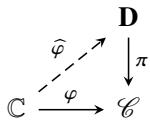
\includegraphics[width=0.7\textwidth]{images/analysis/3da3b3f997e18f24d707369e51b6a777cebf66a347958437b0414fc6788e7463.jpg}
  \\
  \captionof{figure}{Commutative diagram for holomorphic map lifting.}
\end{center}

\begin{exercise}
Let $f$ and $g$ be two holomorphic functions defined on the entire complex plane $\mathbb{C}$ so that for all $z\in\mathbb{C}$, we have
\[
f(z)^{2020} + g(z)^{2020} = 1.
\]
Prove that $f$ and $g$ are constants, see Figure \ref{fig:holomorphic}.

\end{exercise}

\begin{solution}
\textbf{Prerequisites:} 
\begin{itemize}
    \item \textbf{Genus Formula:} For a smooth projective plane curve of degree $n$, the genus is $g = \frac{(n-1)(n-2)}{2}$.
    \item \textbf{Uniformization Theorem:} A simply connected Riemann surface is biholomorphic to the Riemann sphere, $\mathbb{C}$, or the unit disk $\mathbb{D}$. Surfaces with genus $g \geq 2$ have $\mathbb{D}$ as their universal cover.
    \item \textbf{Liouville's Theorem:} A bounded entire function must be constant.
\end{itemize}

\bigskip

\textbf{Steps:}
\begin{enumerate}
    \item \textbf{Define the Curve:} Consider the complex projective curve $\mathcal{C}$ in $\mathbb{P}^2(\mathbb{C})$ defined by the equation:
    \[ z_1^{2020} + z_2^{2020} = z_3^{2020}. \]
    This is a smooth Fermat curve. \\[2ex]

    \item \textbf{Map from $\mathbb{C}$ to $\mathcal{C}$:} Define the holomorphic map $\varphi: \mathbb{C} \to \mathcal{C}$ by $\varphi(z) = [f(z) : g(z) : 1]$. This is well-defined because $f$ and $g$ are entire and satisfy the Fermat equation. \\[2ex]

    \item \textbf{Calculate the Genus:} Using the genus formula for $n=2020$:
    \[ g(\mathcal{C}) = \frac{(2020-1)(2020-2)}{2} = \frac{2019 \times 2018}{2} > 1. \]
    Since $g \geq 2$, the curve $\mathcal{C}$ is a hyperbolic Riemann surface. \\[2ex]

    \item \textbf{Lift to the Universal Cover:} By the Uniformization Theorem, the universal cover of $\mathcal{C}$ is the unit disk $\mathbb{D}$. Since $\mathbb{C}$ is simply connected, any map $\varphi: \mathbb{C} \to \mathcal{C}$ can be lifted to a holomorphic map $\widehat{\varphi}: \mathbb{C} \to \mathbb{D}$ such that $\pi \circ \widehat{\varphi} = \varphi$. \\[2ex]

    \item \textbf{Apply Liouville's Theorem:} The lifted map $\widehat{\varphi}$ is an entire function whose image is contained in the bounded disk $\mathbb{D}$. By Liouville's Theorem, $\widehat{\varphi}$ must be constant. Thus, $\varphi$ is constant, which implies $f$ and $g$ are constants.
\end{enumerate}

\bigskip

\textbf{Intuition:} 
Imagine the equation $f^n + g^n = 1$ as defining a "surface" with many holes (like a multi-holed donut). If $n$ is large, the surface is very "curvy" (hyperbolic). Holomorphic maps from the flat complex plane $\mathbb{C}$ like to stay "flat." Trying to wrap the flat plane onto a very curvy surface without creating "tears" or "stretching" (which holomorphic maps forbid) is impossible unless you just map everything to a single point.
\end{solution}

\begin{exercise}
We consider the following ordinary differential equation:
\[
\begin{cases}
x''(t) + x(t) + x(t)^3 = 0,\\
(x(0),x'(0)) = (x_0,0),
\end{cases}
\]
where $x(t)$ takes values in $\mathbb{R}$. Prove that for all $x_0\in\mathbb{R}$, the solution of the above system is periodic.

\end{exercise}

\begin{solution}
\textbf{Prerequisites:} 
\begin{itemize}
    \item \textbf{Hamiltonian Systems:} Systems where the total energy $E = \text{Kinetic} + \text{Potential}$ is conserved.
    \item \textbf{Phase Plane Analysis:} Studying trajectories in the $(x, x')$ plane.
    \item \textbf{Existence and Uniqueness:} Smooth autonomous systems have unique solutions defined globally if the level sets of the energy are compact.
\end{itemize}

\bigskip

\textbf{Steps:}
\begin{enumerate}
    \item \textbf{Find the Conserved Energy:} Multiply the ODE by $x'(t)$ and integrate:
    \[ x'x'' + x'x + x'x^3 = 0 \implies \frac{d}{dt} \left( \frac{1}{2}(x')^2 + \frac{1}{2}x^2 + \frac{1}{4}x^4 \right) = 0. \]
    The energy $E(x, x') = \frac{1}{2}(x')^2 + \frac{1}{2}x^2 + \frac{1}{4}x^4$ is constant. \\[2ex]

    \item \textbf{Identify the Trajectory:} For the initial condition $(x_0, 0)$, the energy is $E_0 = \frac{1}{2}x_0^2 + \frac{1}{4}x_0^4$. The trajectory in the phase plane $(x, \xi)$ (where $\xi = x'$) is the level set:
    \[ \frac{1}{2}\xi^2 + \frac{1}{2}x^2 + \frac{1}{4}x^4 = E_0. \] \\[2ex]

    \item \textbf{Analyze the Level Set Geometry:} The function $V(x) = \frac{1}{2}x^2 + \frac{1}{4}x^4$ is a potential well. It is strictly convex, has a minimum at $x=0$, and $V(x) \to \infty$ as $|x| \to \infty$. Thus, the level set is a simple, closed, bounded curve (an oval) surrounding the origin. \\[2ex]

    \item \textbf{Prove Periodicity:} Any trajectory on a closed, bounded level set in the phase plane that contains no equilibrium points (except the origin) must be a periodic orbit. The origin $(0,0)$ is the only equilibrium. For any $x_0 \neq 0$, the particle moves along this closed loop and must return to its starting position $(x_0, 0)$. \\[2ex]

    \item \textbf{Alternative Monotonicity Argument:} If the solution were not periodic, $x(t)$ would have to approach a limit or go to infinity. But $x(t)$ is bounded by the energy constraint, and if it doesn't return to the maximum, it would have to be monotone, which contradicts the oscillating nature of the force $-x-x^3$.
\end{enumerate}

\bigskip

\textbf{Intuition:} 
This equation describes a mass on a "nonlinear spring." Unlike a standard spring ($F = -kx$), this spring gets much stiffer as you stretch it further ($F = -x - x^3$). Because there is no friction (no term with $x'$), the energy you put in at the start is never lost. The mass just sloshes back and forth in the "potential bowl" forever, repeating the same motion over and over.
\end{solution}

\begin{exercise}
Let $\alpha\in\mathbb{R}$ and $a_k\in\mathbb{C}$ with $|a_k|<1$, where $k=1,2,\ldots,n$. We consider the following holomorphic map
\[
f:\mathbb{C}\setminus\{(\overline{a_1})^{-1},\dots,(\overline{a_n})^{-1}\}\to\mathbb{C},\quad z\mapsto f(z) = e^{2\sqrt{-1}\pi\alpha}z\cdot\frac{z-a_1}{1-\overline{a_1}z}\cdots\frac{z-a_n}{1-\overline{a_n}z}.
\]

Let $\mathbb{S}^1$ be the unit circle in $\mathbb{C}$, i.e., $\mathbb{S}^1 = \{z\in\mathbb{C}\mid |z|=1\}$.

Prove that $f$ maps $\mathbb{S}^1$ to itself and $f$ preserves the surface measure of $\mathbb{S}^1$.

\end{exercise}

\begin{solution}
\textbf{Prerequisites:} 
\begin{itemize}
    \item \textbf{Blaschke Products:} Functions of the form $B(z) = \prod \frac{z-a_k}{1-\bar{a}_k z}$, which map the unit disk to itself and the unit circle to itself.
    \item \textbf{Mean Value Property for Harmonic Functions:} If $u$ is harmonic, $u(0) = \frac{1}{2\pi} \int_0^{2\pi} u(e^{i\theta}) \, d\theta$.
    \item \textbf{Dirichlet Problem:} Finding a harmonic function on a domain with given values on the boundary.
\end{itemize}

\bigskip

\textbf{Steps:}
\begin{enumerate}
    \item \textbf{Verify Invariance of $\mathbb{S}^1$:} For any $|z|=1$, we have $|1-\bar{a}_k z| = |z(\bar{z}-\bar{a}_k)| = |z||\overline{z-a_k}| = |z-a_k|$.
    Thus, each factor $\left| \frac{z-a_k}{1-\bar{a}_k z} \right| = 1$. Combined with $|e^{2\pi i \alpha}| = 1$ and $|z|=1$, we have $|f(z)|=1$. \\[2ex]

    \item \textbf{Setup the Integral Equality:} To show $f$ preserves measure, we must show $\int_{\mathbb{S}^1} \varphi(f(z)) \, d\theta = \int_{\mathbb{S}^1} \varphi(z) \, d\theta$ for any continuous function $\varphi$. \\[2ex]

    \item \textbf{Extend $\varphi$ Harmonically:} Let $\bar{\varphi}$ be the unique harmonic extension of $\varphi$ from the circle $\mathbb{S}^1$ to the disk $\mathbb{D}$. By the Mean Value Property:
    \[ \int_{\mathbb{S}^1} \varphi(z) \, d\theta = 2\pi \bar{\varphi}(0). \] \\[2ex]

    \item \textbf{Compose with the Holomorphic Map:} Since $f$ is holomorphic and maps the disk $\mathbb{D}$ to itself, the composition $\bar{\varphi} \circ f$ is still a harmonic function on $\mathbb{D}$. Its boundary values on $\mathbb{S}^1$ are exactly $\varphi \circ f$. \\[2ex]

    \item \textbf{Apply Mean Value Property to the Composition:}
    \[ \int_{\mathbb{S}^1} (\varphi \circ f)(z) \, d\theta = 2\pi (\bar{\varphi} \circ f)(0). \]
    Since the map $f$ contains a factor of $z$, we have $f(0) = 0$. Thus:
    \[ 2\pi \bar{\varphi}(f(0)) = 2\pi \bar{\varphi}(0). \]
    This matches the original integral, so the measure is preserved.
\end{enumerate}

\bigskip

\textbf{Intuition:} 
Think of the unit circle as a looped string and $f$ as a way of rearranging or "winding" the string onto itself. The map $f$ is like a high-quality "shuffling" machine. Because $f(0)=0$, it means the "center of mass" of the circle doesn't shift. The property of being "harmonic" means that the average value on the boundary is determined solely by the value at the center. Since $f$ keeps the center at the center, it doesn't change the average value of any function, which is the definition of preserving measure.
\end{solution}
